\documentclass[1p]{elsarticle_modified}
%\bibliographystyle{elsarticle-num}

%\usepackage[colorlinks]{hyperref}
%\usepackage{abbrmath_seonhwa} %\Abb, \Ascr, \Acal ,\Abf, \Afrak
\usepackage{amsfonts}
\usepackage{amssymb}
\usepackage{amsmath}
\usepackage{amsthm}
\usepackage{scalefnt}
\usepackage{amsbsy}
\usepackage{kotex}
\usepackage{caption}
\usepackage{subfig}
\usepackage{color}
\usepackage{graphicx}
\usepackage{xcolor} %% white, black, red, green, blue, cyan, magenta, yellow
\usepackage{float}
\usepackage{setspace}
\usepackage{hyperref}

\usepackage{tikz}
\usetikzlibrary{arrows}

\usepackage{multirow}
\usepackage{array} % fixed length table
\usepackage{hhline}

%%%%%%%%%%%%%%%%%%%%%
\makeatletter
\renewcommand*\env@matrix[1][\arraystretch]{%
	\edef\arraystretch{#1}%
	\hskip -\arraycolsep
	\let\@ifnextchar\new@ifnextchar
	\array{*\c@MaxMatrixCols c}}
\makeatother %https://tex.stackexchange.com/questions/14071/how-can-i-increase-the-line-spacing-in-a-matrix
%%%%%%%%%%%%%%%

\usepackage[normalem]{ulem}

\newcommand{\msout}[1]{\ifmmode\text{\sout{\ensuremath{#1}}}\else\sout{#1}\fi}
%SOURCE: \msout is \stkout macro in https://tex.stackexchange.com/questions/20609/strikeout-in-math-mode

\newcommand{\cancel}[1]{
	\ifmmode
	{\color{red}\msout{#1}}
	\else
	{\color{red}\sout{#1}}
	\fi
}

\newcommand{\add}[1]{
	{\color{blue}\uwave{#1}}
}

\newcommand{\replace}[2]{
	\ifmmode
	{\color{red}\msout{#1}}{\color{blue}\uwave{#2}}
	\else
	{\color{red}\sout{#1}}{\color{blue}\uwave{#2}}
	\fi
}

\newcommand{\Sol}{\mathcal{S}} %segment
\newcommand{\D}{D} %diagram
\newcommand{\A}{\mathcal{A}} %arc


%%%%%%%%%%%%%%%%%%%%%%%%%%%%%5 test

\def\sl{\operatorname{\textup{SL}}(2,\Cbb)}
\def\psl{\operatorname{\textup{PSL}}(2,\Cbb)}
\def\quan{\mkern 1mu \triangleright \mkern 1mu}

\theoremstyle{definition}
\newtheorem{thm}{Theorem}[section]
\newtheorem{prop}[thm]{Proposition}
\newtheorem{lem}[thm]{Lemma}
\newtheorem{ques}[thm]{Question}
\newtheorem{cor}[thm]{Corollary}
\newtheorem{defn}[thm]{Definition}
\newtheorem{exam}[thm]{Example}
\newtheorem{rmk}[thm]{Remark}
\newtheorem{alg}[thm]{Algorithm}

\newcommand{\I}{\sqrt{-1}}
\begin{document}

%\begin{frontmatter}
%
%\title{Boundary parabolic representations of knots up to 8 crossings}
%
%%% Group authors per affiliation:
%\author{Yunhi Cho} 
%\address{Department of Mathematics, University of Seoul, Seoul, Korea}
%\ead{yhcho@uos.ac.kr}
%
%
%\author{Seonhwa Kim} %\fnref{s_kim}}
%\address{Center for Geometry and Physics, Institute for Basic Science, Pohang, 37673, Korea}
%\ead{ryeona17@ibs.re.kr}
%
%\author{Hyuk Kim}
%\address{Department of Mathematical Sciences, Seoul National University, Seoul 08826, Korea}
%\ead{hyukkim@snu.ac.kr}
%
%\author{Seokbeom Yoon}
%\address{Department of Mathematical Sciences, Seoul National University, Seoul, 08826,  Korea}
%\ead{sbyoon15@snu.ac.kr}
%
%\begin{abstract}
%We find all boundary parabolic representation of knots up to 8 crossings.
%
%\end{abstract}
%\begin{keyword}
%    \MSC[2010] 57M25 
%\end{keyword}
%
%\end{frontmatter}

%\linenumbers
%\tableofcontents
%
\newcommand\colored[1]{\textcolor{white}{\rule[-0.35ex]{0.8em}{1.4ex}}\kern-0.8em\color{red} #1}%
%\newcommand\colored[1]{\textcolor{white}{ #1}\kern-2.17ex	\textcolor{white}{ #1}\kern-1.81ex	\textcolor{white}{ #1}\kern-2.15ex\color{red}#1	}

{\Large $\underline{12a_{1013}~(K12a_{1013})}$}

\setlength{\tabcolsep}{10pt}
\renewcommand{\arraystretch}{1.6}
\vspace{1cm}\begin{tabular}{m{100pt}>{\centering\arraybackslash}m{274pt}}
\multirow{5}{120pt}{
	\centering
	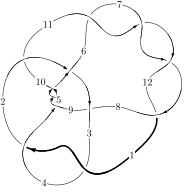
\includegraphics[width=112pt]{../../../GIT/diagram.site/Diagrams/png/1814_12a_1013.png}\\
\ \ \ A knot diagram\footnotemark}&
\allowdisplaybreaks
\textbf{Linearized knot diagam} \\
\cline{2-2}
 &
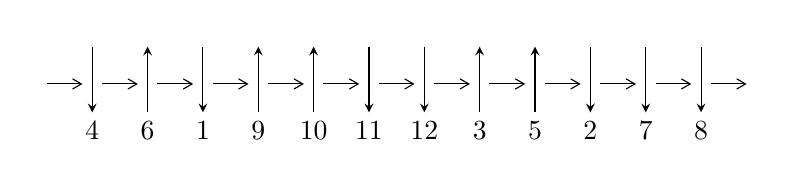
\begin{tikzpicture}[x=20pt, y=17pt]
	% nodes
	\node (C0) at (0, 0) {};
	\node (C1) at (1, 0) {};
	\node (C1U) at (1, +1) {};
	\node (C1D) at (1, -1) {4};

	\node (C2) at (2, 0) {};
	\node (C2U) at (2, +1) {};
	\node (C2D) at (2, -1) {6};

	\node (C3) at (3, 0) {};
	\node (C3U) at (3, +1) {};
	\node (C3D) at (3, -1) {1};

	\node (C4) at (4, 0) {};
	\node (C4U) at (4, +1) {};
	\node (C4D) at (4, -1) {9};

	\node (C5) at (5, 0) {};
	\node (C5U) at (5, +1) {};
	\node (C5D) at (5, -1) {10};

	\node (C6) at (6, 0) {};
	\node (C6U) at (6, +1) {};
	\node (C6D) at (6, -1) {11};

	\node (C7) at (7, 0) {};
	\node (C7U) at (7, +1) {};
	\node (C7D) at (7, -1) {12};

	\node (C8) at (8, 0) {};
	\node (C8U) at (8, +1) {};
	\node (C8D) at (8, -1) {3};

	\node (C9) at (9, 0) {};
	\node (C9U) at (9, +1) {};
	\node (C9D) at (9, -1) {5};

	\node (C10) at (10, 0) {};
	\node (C10U) at (10, +1) {};
	\node (C10D) at (10, -1) {2};

	\node (C11) at (11, 0) {};
	\node (C11U) at (11, +1) {};
	\node (C11D) at (11, -1) {7};

	\node (C12) at (12, 0) {};
	\node (C12U) at (12, +1) {};
	\node (C12D) at (12, -1) {8};
	\node (C13) at (13, 0) {};

	% arrows
	\draw[->,>={angle 60}]
	(C0) edge (C1) (C1) edge (C2) (C2) edge (C3) (C3) edge (C4) (C4) edge (C5) (C5) edge (C6) (C6) edge (C7) (C7) edge (C8) (C8) edge (C9) (C9) edge (C10) (C10) edge (C11) (C11) edge (C12) (C12) edge (C13) ;	\draw[->,>=stealth]
	(C1U) edge (C1D) (C2D) edge (C2U) (C3U) edge (C3D) (C4D) edge (C4U) (C5D) edge (C5U) (C6U) edge (C6D) (C7U) edge (C7D) (C8D) edge (C8U) (C9D) edge (C9U) (C10U) edge (C10D) (C11U) edge (C11D) (C12U) edge (C12D) ;
	\end{tikzpicture} \\
\hhline{~~} \\& 
\textbf{Solving Sequence} \\ \cline{2-2} 
 &
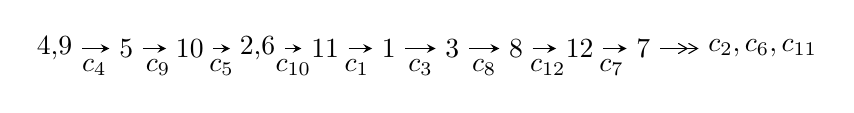
\begin{tikzpicture}[x=23pt, y=7pt]
	% node
	\node (A0) at (-1/8, 0) {4,9};
	\node (A1) at (1, 0) {5};
	\node (A2) at (2, 0) {10};
	\node (A3) at (49/16, 0) {2,6};
	\node (A4) at (33/8, 0) {11};
	\node (A5) at (41/8, 0) {1};
	\node (A6) at (49/8, 0) {3};
	\node (A7) at (57/8, 0) {8};
	\node (A8) at (65/8, 0) {12};
	\node (A9) at (73/8, 0) {7};
	\node (C1) at (1/2, -1) {$c_{4}$};
	\node (C2) at (3/2, -1) {$c_{9}$};
	\node (C3) at (5/2, -1) {$c_{5}$};
	\node (C4) at (29/8, -1) {$c_{10}$};
	\node (C5) at (37/8, -1) {$c_{1}$};
	\node (C6) at (45/8, -1) {$c_{3}$};
	\node (C7) at (53/8, -1) {$c_{8}$};
	\node (C8) at (61/8, -1) {$c_{12}$};
	\node (C9) at (69/8, -1) {$c_{7}$};
	\node (A10) at (11, 0) {$c_{2},c_{6},c_{11}$};

	% edge
	\draw[->,>=stealth]	
	(A0) edge (A1) (A1) edge (A2) (A2) edge (A3) (A3) edge (A4) (A4) edge (A5) (A5) edge (A6) (A6) edge (A7) (A7) edge (A8) (A8) edge (A9) ;
	\draw[->>,>={angle 60}]	
	(A9) edge (A10);
\end{tikzpicture} \\ 

\end{tabular} \\

\footnotetext{
The image of knot diagram is generated by the software ``\textbf{Draw programme}" developed by Andrew Bartholomew(\url{http://www.layer8.co.uk/maths/draw/index.htm\#Running-draw}), where we modified some parts for our purpose(\url{https://github.com/CATsTAILs/LinksPainter}).
}\phantom \\ \newline 
\centering \textbf{Ideals for irreducible components\footnotemark of $X_{\text{par}}$} 
 
\begin{align*}
I^u_{1}&=\langle 
-6.11706\times10^{59} u^{58}+1.07231\times10^{60} u^{57}+\cdots+4.86975\times10^{59} b+9.72469\times10^{59},\\
\phantom{I^u_{1}}&\phantom{= \langle  }-2.05091\times10^{60} u^{58}+3.51655\times10^{60} u^{57}+\cdots+4.86975\times10^{59} a+1.34143\times10^{60},\;u^{59}-3 u^{58}+\cdots+3 u^2+1\rangle \\
\\
\end{align*}
\raggedright * 1 irreducible components of $\dim_{\mathbb{C}}=0$, with total 59 representations.\\
\footnotetext{All coefficients of polynomials are rational numbers. But the coefficients are sometimes approximated in decimal forms when there is not enough margin.}
\newpage
\renewcommand{\arraystretch}{1}
\centering \section*{I. $I^u_{1}= \langle -6.12\times10^{59} u^{58}+1.07\times10^{60} u^{57}+\cdots+4.87\times10^{59} b+9.72\times10^{59},\;-2.05\times10^{60} u^{58}+3.52\times10^{60} u^{57}+\cdots+4.87\times10^{59} a+1.34\times10^{60},\;u^{59}-3 u^{58}+\cdots+3 u^2+1 \rangle$}
\flushleft \textbf{(i) Arc colorings}\\
\begin{tabular}{m{7pt} m{180pt} m{7pt} m{180pt} }
\flushright $a_{4}=$&$\begin{pmatrix}1\\0\end{pmatrix}$ \\
\flushright $a_{9}=$&$\begin{pmatrix}0\\u\end{pmatrix}$ \\
\flushright $a_{5}=$&$\begin{pmatrix}1\\- u^2\end{pmatrix}$ \\
\flushright $a_{10}=$&$\begin{pmatrix}u\\- u^3+u\end{pmatrix}$ \\
\flushright $a_{2}=$&$\begin{pmatrix}4.21152 u^{58}-7.22122 u^{57}+\cdots-12.4594 u-2.75461\\1.25613 u^{58}-2.20198 u^{57}+\cdots-0.819175 u-1.99696\end{pmatrix}$ \\
\flushright $a_{6}=$&$\begin{pmatrix}- u^2+1\\u^4-2 u^2\end{pmatrix}$ \\
\flushright $a_{11}=$&$\begin{pmatrix}-9.15963 u^{58}+16.8081 u^{57}+\cdots+1.60609 u+10.4724\\-6.32014 u^{58}+10.8093 u^{57}+\cdots+5.10432 u+4.56009\end{pmatrix}$ \\
\flushright $a_{1}=$&$\begin{pmatrix}5.46765 u^{58}-9.42320 u^{57}+\cdots-13.2786 u-4.75157\\1.25613 u^{58}-2.20198 u^{57}+\cdots-0.819175 u-1.99696\end{pmatrix}$ \\
\flushright $a_{3}=$&$\begin{pmatrix}4.39790 u^{58}-7.52436 u^{57}+\cdots-12.3770 u-2.98622\\1.32770 u^{58}-2.27810 u^{57}+\cdots-0.861136 u-2.06309\end{pmatrix}$ \\
\flushright $a_{8}=$&$\begin{pmatrix}12.1066 u^{58}-24.6727 u^{57}+\cdots-15.8303 u-1.97288\\4.64955 u^{58}-6.59987 u^{57}+\cdots-1.46326 u-3.70154\end{pmatrix}$ \\
\flushright $a_{12}=$&$\begin{pmatrix}10.5375 u^{58}-10.9059 u^{57}+\cdots-11.6889 u-15.2433\\0.324061 u^{58}-0.967105 u^{57}+\cdots-0.188037 u-0.274138\end{pmatrix}$ \\
\flushright $a_{7}=$&$\begin{pmatrix}8.66021 u^{58}-9.05645 u^{57}+\cdots-8.23792 u-4.80111\\0.825077 u^{58}-1.28802 u^{57}+\cdots-0.769376 u-1.21854\end{pmatrix}$\\&\end{tabular}
\flushleft \textbf{(ii) Obstruction class $= -1$}\\~\\
\flushleft \textbf{(iii) Cusp Shapes $= -26.5735 u^{58}+37.2947 u^{57}+\cdots+9.09129 u+20.6511$}\\~\\
\newpage\renewcommand{\arraystretch}{1}
\flushleft \textbf{(iv) u-Polynomials at the component}\newline \\
\begin{tabular}{m{50pt}|m{274pt}}
Crossings & \hspace{64pt}u-Polynomials at each crossing \\
\hline $$\begin{aligned}c_{1},c_{3}\end{aligned}$$&$\begin{aligned}
&u^{59}- u^{58}+\cdots-46 u+1
\end{aligned}$\\
\hline $$\begin{aligned}c_{2}\end{aligned}$$&$\begin{aligned}
&u^{59}-5 u^{58}+\cdots+4 u+1
\end{aligned}$\\
\hline $$\begin{aligned}c_{4},c_{5},c_{9}\end{aligned}$$&$\begin{aligned}
&u^{59}+3 u^{58}+\cdots-3 u^2-1
\end{aligned}$\\
\hline $$\begin{aligned}c_{6},c_{7},c_{11}\\c_{12}\end{aligned}$$&$\begin{aligned}
&u^{59}- u^{58}+\cdots+3 u^2+1
\end{aligned}$\\
\hline $$\begin{aligned}c_{8}\end{aligned}$$&$\begin{aligned}
&u^{59}-49 u^{58}+\cdots+67362 u-16529
\end{aligned}$\\
\hline $$\begin{aligned}c_{10}\end{aligned}$$&$\begin{aligned}
&u^{59}+53 u^{58}+\cdots+256 u+19
\end{aligned}$\\
\hline
\end{tabular}\\~\\
\newpage\renewcommand{\arraystretch}{1}
\flushleft \textbf{(v) Riley Polynomials at the component}\newline \\
\begin{tabular}{m{50pt}|m{274pt}}
Crossings & \hspace{64pt}Riley Polynomials at each crossing \\
\hline $$\begin{aligned}c_{1},c_{3}\end{aligned}$$&$\begin{aligned}
&y^{59}-41 y^{58}+\cdots+1910 y-1
\end{aligned}$\\
\hline $$\begin{aligned}c_{2}\end{aligned}$$&$\begin{aligned}
&y^{59}+3 y^{58}+\cdots+270 y-1
\end{aligned}$\\
\hline $$\begin{aligned}c_{4},c_{5},c_{9}\end{aligned}$$&$\begin{aligned}
&y^{59}-57 y^{58}+\cdots-6 y-1
\end{aligned}$\\
\hline $$\begin{aligned}c_{6},c_{7},c_{11}\\c_{12}\end{aligned}$$&$\begin{aligned}
&y^{59}-73 y^{58}+\cdots-6 y-1
\end{aligned}$\\
\hline $$\begin{aligned}c_{8}\end{aligned}$$&$\begin{aligned}
&y^{59}-2169 y^{58}+\cdots+18247485862 y-273207841
\end{aligned}$\\
\hline $$\begin{aligned}c_{10}\end{aligned}$$&$\begin{aligned}
&y^{59}-2137 y^{58}+\cdots+12906 y-361
\end{aligned}$\\
\hline
\end{tabular}\\~\\
\newpage\flushleft \textbf{(vi) Complex Volumes and Cusp Shapes}
$$\begin{array}{c|c|c}  
\text{Solutions to }I^u_{1}& \I (\text{vol} + \sqrt{-1}CS) & \text{Cusp shape}\\
 \hline 
\begin{aligned}
u &= \phantom{-}0.475350 + 0.860447 I \\
a &= \phantom{-}0.496568 + 0.839468 I \\
b &= \phantom{-}1.272020 - 0.381627 I\end{aligned}
 & -5.19566 + 7.84726 I & \phantom{-0.000000 } 0 \\ \hline\begin{aligned}
u &= \phantom{-}0.475350 - 0.860447 I \\
a &= \phantom{-}0.496568 - 0.839468 I \\
b &= \phantom{-}1.272020 + 0.381627 I\end{aligned}
 & -5.19566 - 7.84726 I & \phantom{-0.000000 } 0 \\ \hline\begin{aligned}
u &= -0.496786 + 0.831191 I \\
a &= \phantom{-}0.452243 - 1.016940 I \\
b &= \phantom{-}1.41446 + 0.46980 I\end{aligned}
 & -14.4117 - 10.5302 I & \phantom{-0.000000 } 0 \\ \hline\begin{aligned}
u &= -0.496786 - 0.831191 I \\
a &= \phantom{-}0.452243 + 1.016940 I \\
b &= \phantom{-}1.41446 - 0.46980 I\end{aligned}
 & -14.4117 + 10.5302 I & \phantom{-0.000000 } 0 \\ \hline\begin{aligned}
u &= -0.642055 + 0.817094 I \\
a &= -0.098059 - 0.497244 I \\
b &= \phantom{-}1.325190 - 0.298324 I\end{aligned}
 & -14.0087 + 5.0802 I & \phantom{-0.000000 } 0 \\ \hline\begin{aligned}
u &= -0.642055 - 0.817094 I \\
a &= -0.098059 + 0.497244 I \\
b &= \phantom{-}1.325190 + 0.298324 I\end{aligned}
 & -14.0087 - 5.0802 I & \phantom{-0.000000 } 0 \\ \hline\begin{aligned}
u &= -0.439918 + 0.966336 I \\
a &= \phantom{-}0.481104 - 0.534588 I \\
b &= \phantom{-}1.100680 + 0.202044 I\end{aligned}
 & -1.85929 - 3.33269 I & \phantom{-0.000000 } 0 \\ \hline\begin{aligned}
u &= -0.439918 - 0.966336 I \\
a &= \phantom{-}0.481104 + 0.534588 I \\
b &= \phantom{-}1.100680 - 0.202044 I\end{aligned}
 & -1.85929 + 3.33269 I & \phantom{-0.000000 } 0 \\ \hline\begin{aligned}
u &= \phantom{-}1.13498\phantom{ +0.000000I} \\
a &= \phantom{-}0.740239\phantom{ +0.000000I} \\
b &= \phantom{-}0.378809\phantom{ +0.000000I}\end{aligned}
 & -4.07948\phantom{ +0.000000I} & \phantom{-0.000000 } 0 \\ \hline\begin{aligned}
u &= \phantom{-}0.727904 + 0.915102 I \\
a &= \phantom{-}0.087669 + 0.413864 I \\
b &= \phantom{-}1.132370 + 0.126938 I\end{aligned}
 & -4.55152 - 2.10422 I & \phantom{-0.000000 } 0\\
 \hline 
 \end{array}$$\newpage$$\begin{array}{c|c|c}  
\text{Solutions to }I^u_{1}& \I (\text{vol} + \sqrt{-1}CS) & \text{Cusp shape}\\
 \hline 
\begin{aligned}
u &= \phantom{-}0.727904 - 0.915102 I \\
a &= \phantom{-}0.087669 - 0.413864 I \\
b &= \phantom{-}1.132370 - 0.126938 I\end{aligned}
 & -4.55152 + 2.10422 I & \phantom{-0.000000 } 0 \\ \hline\begin{aligned}
u &= \phantom{-}1.21857\phantom{ +0.000000I} \\
a &= \phantom{-}1.69323\phantom{ +0.000000I} \\
b &= -1.89392\phantom{ +0.000000I}\end{aligned}
 & -10.6108\phantom{ +0.000000I} & \phantom{-0.000000 } 0 \\ \hline\begin{aligned}
u &= -1.26436\phantom{ +0.000000I} \\
a &= \phantom{-}1.11134\phantom{ +0.000000I} \\
b &= -1.65979\phantom{ +0.000000I}\end{aligned}
 & -1.59640\phantom{ +0.000000I} & \phantom{-0.000000 } 0 \\ \hline\begin{aligned}
u &= -1.316980 + 0.152107 I \\
a &= \phantom{-}1.03120 + 1.96585 I \\
b &= -1.40555 - 1.05122 I\end{aligned}
 & -8.95609 - 4.55404 I & \phantom{-0.000000 } 0 \\ \hline\begin{aligned}
u &= -1.316980 - 0.152107 I \\
a &= \phantom{-}1.03120 - 1.96585 I \\
b &= -1.40555 + 1.05122 I\end{aligned}
 & -8.95609 + 4.55404 I & \phantom{-0.000000 } 0 \\ \hline\begin{aligned}
u &= -0.381236 + 0.552080 I \\
a &= -0.167585 + 0.667792 I \\
b &= -0.208595 - 1.152770 I\end{aligned}
 & -9.30665 - 4.95113 I & -6.99238 + 6.51896 I \\ \hline\begin{aligned}
u &= -0.381236 - 0.552080 I \\
a &= -0.167585 - 0.667792 I \\
b &= -0.208595 + 1.152770 I\end{aligned}
 & -9.30665 + 4.95113 I & -6.99238 - 6.51896 I \\ \hline\begin{aligned}
u &= \phantom{-}1.334770 + 0.126781 I \\
a &= \phantom{-}0.82384 - 1.77989 I \\
b &= -1.22573 + 0.84622 I\end{aligned}
 & -0.05622 + 3.78887 I & \phantom{-0.000000 } 0 \\ \hline\begin{aligned}
u &= \phantom{-}1.334770 - 0.126781 I \\
a &= \phantom{-}0.82384 + 1.77989 I \\
b &= -1.22573 - 0.84622 I\end{aligned}
 & -0.05622 - 3.78887 I & \phantom{-0.000000 } 0 \\ \hline\begin{aligned}
u &= \phantom{-}0.407640 + 0.491215 I \\
a &= \phantom{-}0.007046 - 0.614145 I \\
b &= -0.124106 + 0.847511 I\end{aligned}
 & -0.95048 + 3.54930 I & -4.43989 - 9.05516 I\\
 \hline 
 \end{array}$$\newpage$$\begin{array}{c|c|c}  
\text{Solutions to }I^u_{1}& \I (\text{vol} + \sqrt{-1}CS) & \text{Cusp shape}\\
 \hline 
\begin{aligned}
u &= \phantom{-}0.407640 - 0.491215 I \\
a &= \phantom{-}0.007046 + 0.614145 I \\
b &= -0.124106 - 0.847511 I\end{aligned}
 & -0.95048 - 3.54930 I & -4.43989 + 9.05516 I \\ \hline\begin{aligned}
u &= \phantom{-}1.364330 + 0.022066 I \\
a &= -1.08977 - 1.29712 I \\
b &= -1.114170 + 0.098313 I\end{aligned}
 & \phantom{-}2.05873 + 0.05448 I & \phantom{-0.000000 } 0 \\ \hline\begin{aligned}
u &= \phantom{-}1.364330 - 0.022066 I \\
a &= -1.08977 + 1.29712 I \\
b &= -1.114170 - 0.098313 I\end{aligned}
 & \phantom{-}2.05873 - 0.05448 I & \phantom{-0.000000 } 0 \\ \hline\begin{aligned}
u &= -1.365210 + 0.084494 I \\
a &= \phantom{-}0.52896 + 1.73722 I \\
b &= -1.000010 - 0.478965 I\end{aligned}
 & \phantom{-}2.93987 - 2.06641 I & \phantom{-0.000000 } 0 \\ \hline\begin{aligned}
u &= -1.365210 - 0.084494 I \\
a &= \phantom{-}0.52896 - 1.73722 I \\
b &= -1.000010 + 0.478965 I\end{aligned}
 & \phantom{-}2.93987 + 2.06641 I & \phantom{-0.000000 } 0 \\ \hline\begin{aligned}
u &= \phantom{-}1.38545\phantom{ +0.000000I} \\
a &= \phantom{-}1.11296\phantom{ +0.000000I} \\
b &= \phantom{-}0.0228314\phantom{ +0.000000I}\end{aligned}
 & -3.92767\phantom{ +0.000000I} & \phantom{-0.000000 } 0 \\ \hline\begin{aligned}
u &= -0.488282 + 0.360464 I \\
a &= \phantom{-}0.329573 + 0.368478 I \\
b &= \phantom{-}0.087132 - 0.424414 I\end{aligned}
 & \phantom{-}0.926561 - 0.875889 I & \phantom{-}4.21577 + 2.97992 I \\ \hline\begin{aligned}
u &= -0.488282 - 0.360464 I \\
a &= \phantom{-}0.329573 - 0.368478 I \\
b &= \phantom{-}0.087132 + 0.424414 I\end{aligned}
 & \phantom{-}0.926561 + 0.875889 I & \phantom{-}4.21577 - 2.97992 I \\ \hline\begin{aligned}
u &= -1.42001\phantom{ +0.000000I} \\
a &= \phantom{-}32.7779\phantom{ +0.000000I} \\
b &= -1.00219\phantom{ +0.000000I}\end{aligned}
 & -5.59723\phantom{ +0.000000I} & \phantom{-0.000000 } 0 \\ \hline\begin{aligned}
u &= -0.367886 + 0.436129 I \\
a &= \phantom{-}2.08179 + 0.08994 I \\
b &= -0.257332 + 0.613928 I\end{aligned}
 & -9.13968 + 1.69764 I & -6.18348 + 2.07569 I\\
 \hline 
 \end{array}$$\newpage$$\begin{array}{c|c|c}  
\text{Solutions to }I^u_{1}& \I (\text{vol} + \sqrt{-1}CS) & \text{Cusp shape}\\
 \hline 
\begin{aligned}
u &= -0.367886 - 0.436129 I \\
a &= \phantom{-}2.08179 - 0.08994 I \\
b &= -0.257332 - 0.613928 I\end{aligned}
 & -9.13968 - 1.69764 I & -6.18348 - 2.07569 I \\ \hline\begin{aligned}
u &= \phantom{-}0.117896 + 0.543965 I \\
a &= -0.454546 - 0.643164 I \\
b &= -1.53639 + 0.58516 I\end{aligned}
 & -13.38520 + 2.05056 I & -13.15743 - 3.37772 I \\ \hline\begin{aligned}
u &= \phantom{-}0.117896 - 0.543965 I \\
a &= -0.454546 + 0.643164 I \\
b &= -1.53639 - 0.58516 I\end{aligned}
 & -13.38520 - 2.05056 I & -13.15743 + 3.37772 I \\ \hline\begin{aligned}
u &= \phantom{-}1.44862 + 0.19565 I \\
a &= -0.40513 - 1.85474 I \\
b &= \phantom{-}0.04576 + 1.43936 I\end{aligned}
 & -3.39872 + 7.68478 I & \phantom{-0.000000 } 0 \\ \hline\begin{aligned}
u &= \phantom{-}1.44862 - 0.19565 I \\
a &= -0.40513 + 1.85474 I \\
b &= \phantom{-}0.04576 - 1.43936 I\end{aligned}
 & -3.39872 - 7.68478 I & \phantom{-0.000000 } 0 \\ \hline\begin{aligned}
u &= -1.46045 + 0.17666 I \\
a &= -0.31469 + 1.57531 I \\
b &= \phantom{-}0.099782 - 1.188640 I\end{aligned}
 & \phantom{-}5.11240 - 6.01691 I & \phantom{-0.000000 } 0 \\ \hline\begin{aligned}
u &= -1.46045 - 0.17666 I \\
a &= -0.31469 - 1.57531 I \\
b &= \phantom{-}0.099782 + 1.188640 I\end{aligned}
 & \phantom{-}5.11240 + 6.01691 I & \phantom{-0.000000 } 0 \\ \hline\begin{aligned}
u &= \phantom{-}1.48347 + 0.15220 I \\
a &= -0.239639 - 1.190530 I \\
b &= \phantom{-}0.220135 + 0.883885 I\end{aligned}
 & \phantom{-}7.36971 + 2.90930 I & \phantom{-0.000000 } 0 \\ \hline\begin{aligned}
u &= \phantom{-}1.48347 - 0.15220 I \\
a &= -0.239639 + 1.190530 I \\
b &= \phantom{-}0.220135 - 0.883885 I\end{aligned}
 & \phantom{-}7.36971 - 2.90930 I & \phantom{-0.000000 } 0 \\ \hline\begin{aligned}
u &= -0.120295 + 0.487779 I \\
a &= -0.692408 + 0.804530 I \\
b &= -1.316860 - 0.433488 I\end{aligned}
 & -4.56753 - 1.60582 I & -13.6627 + 4.6604 I\\
 \hline 
 \end{array}$$\newpage$$\begin{array}{c|c|c}  
\text{Solutions to }I^u_{1}& \I (\text{vol} + \sqrt{-1}CS) & \text{Cusp shape}\\
 \hline 
\begin{aligned}
u &= -0.120295 - 0.487779 I \\
a &= -0.692408 - 0.804530 I \\
b &= -1.316860 + 0.433488 I\end{aligned}
 & -4.56753 + 1.60582 I & -13.6627 - 4.6604 I \\ \hline\begin{aligned}
u &= -1.51362 + 0.08542 I \\
a &= \phantom{-}0.043229 + 0.571042 I \\
b &= \phantom{-}0.282289 - 0.378928 I\end{aligned}
 & \phantom{-}4.55593 - 0.22771 I & \phantom{-0.000000 } 0 \\ \hline\begin{aligned}
u &= -1.51362 - 0.08542 I \\
a &= \phantom{-}0.043229 - 0.571042 I \\
b &= \phantom{-}0.282289 + 0.378928 I\end{aligned}
 & \phantom{-}4.55593 + 0.22771 I & \phantom{-0.000000 } 0 \\ \hline\begin{aligned}
u &= \phantom{-}0.471023\phantom{ +0.000000I} \\
a &= \phantom{-}4.79719\phantom{ +0.000000I} \\
b &= -1.27746\phantom{ +0.000000I}\end{aligned}
 & -11.4096\phantom{ +0.000000I} & \phantom{-}1.93000\phantom{ +0.000000I} \\ \hline\begin{aligned}
u &= \phantom{-}1.49877 + 0.32931 I \\
a &= -0.218270 + 1.315670 I \\
b &= \phantom{-}1.192200 - 0.489021 I\end{aligned}
 & \phantom{-}4.33779 + 7.88058 I & \phantom{-0.000000 } 0 \\ \hline\begin{aligned}
u &= \phantom{-}1.49877 - 0.32931 I \\
a &= -0.218270 - 1.315670 I \\
b &= \phantom{-}1.192200 + 0.489021 I\end{aligned}
 & \phantom{-}4.33779 - 7.88058 I & \phantom{-0.000000 } 0 \\ \hline\begin{aligned}
u &= -1.48704 + 0.38777 I \\
a &= -0.131122 - 0.943356 I \\
b &= \phantom{-}1.072210 + 0.305514 I\end{aligned}
 & \phantom{-}2.27021 - 3.30917 I & \phantom{-0.000000 } 0 \\ \hline\begin{aligned}
u &= -1.48704 - 0.38777 I \\
a &= -0.131122 + 0.943356 I \\
b &= \phantom{-}1.072210 - 0.305514 I\end{aligned}
 & \phantom{-}2.27021 + 3.30917 I & \phantom{-0.000000 } 0 \\ \hline\begin{aligned}
u &= \phantom{-}0.261111 + 0.381583 I \\
a &= \phantom{-}1.47093 - 0.33575 I \\
b &= -0.143895 - 0.219363 I\end{aligned}
 & -1.184200 - 0.687771 I & -5.69781 + 0.37912 I \\ \hline\begin{aligned}
u &= \phantom{-}0.261111 - 0.381583 I \\
a &= \phantom{-}1.47093 + 0.33575 I \\
b &= -0.143895 + 0.219363 I\end{aligned}
 & -1.184200 + 0.687771 I & -5.69781 - 0.37912 I\\
 \hline 
 \end{array}$$\newpage$$\begin{array}{c|c|c}  
\text{Solutions to }I^u_{1}& \I (\text{vol} + \sqrt{-1}CS) & \text{Cusp shape}\\
 \hline 
\begin{aligned}
u &= -1.51346 + 0.31095 I \\
a &= -0.38347 - 1.52566 I \\
b &= \phantom{-}1.32664 + 0.57039 I\end{aligned}
 & \phantom{-}1.22146 - 12.09350 I & \phantom{-0.000000 } 0 \\ \hline\begin{aligned}
u &= -1.51346 - 0.31095 I \\
a &= -0.38347 + 1.52566 I \\
b &= \phantom{-}1.32664 - 0.57039 I\end{aligned}
 & \phantom{-}1.22146 + 12.09350 I & \phantom{-0.000000 } 0 \\ \hline\begin{aligned}
u &= \phantom{-}1.52191 + 0.30160 I \\
a &= -0.52248 + 1.67114 I \\
b &= \phantom{-}1.43503 - 0.62232 I\end{aligned}
 & -7.8780 + 14.6651 I & \phantom{-0.000000 } 0 \\ \hline\begin{aligned}
u &= \phantom{-}1.52191 - 0.30160 I \\
a &= -0.52248 - 1.67114 I \\
b &= \phantom{-}1.43503 + 0.62232 I\end{aligned}
 & -7.8780 - 14.6651 I & \phantom{-0.000000 } 0 \\ \hline\begin{aligned}
u &= \phantom{-}0.131491 + 0.330288 I \\
a &= -1.50228 - 2.45162 I \\
b &= -1.005580 + 0.138537 I\end{aligned}
 & -1.78580 + 0.58489 I & -5.41482 + 2.56044 I \\ \hline\begin{aligned}
u &= \phantom{-}0.131491 - 0.330288 I \\
a &= -1.50228 + 2.45162 I \\
b &= -1.005580 - 0.138537 I\end{aligned}
 & -1.78580 - 0.58489 I & -5.41482 - 2.56044 I \\ \hline\begin{aligned}
u &= -0.340698\phantom{ +0.000000I} \\
a &= \phantom{-}6.50413\phantom{ +0.000000I} \\
b &= -1.09163\phantom{ +0.000000I}\end{aligned}
 & -2.98842\phantom{ +0.000000I} & \phantom{-}17.3980\phantom{ +0.000000I} \\ \hline\begin{aligned}
u &= \phantom{-}1.72747 + 0.35363 I \\
a &= -0.483202 + 0.301946 I \\
b &= \phantom{-}1.093980 + 0.049807 I\end{aligned}
 & -6.28102 - 0.67182 I & \phantom{-0.000000 } 0 \\ \hline\begin{aligned}
u &= \phantom{-}1.72747 - 0.35363 I \\
a &= -0.483202 - 0.301946 I \\
b &= \phantom{-}1.093980 - 0.049807 I\end{aligned}
 & -6.28102 + 0.67182 I & \phantom{-0.000000 } 0\\
 \hline 
 \end{array}$$\newpage
\newpage\renewcommand{\arraystretch}{1}
\centering \section*{ II. u-Polynomials}
\begin{tabular}{m{50pt}|m{274pt}}
Crossings & \hspace{64pt}u-Polynomials at each crossing \\
\hline $$\begin{aligned}c_{1},c_{3}\end{aligned}$$&$\begin{aligned}
&u^{59}- u^{58}+\cdots-46 u+1
\end{aligned}$\\
\hline $$\begin{aligned}c_{2}\end{aligned}$$&$\begin{aligned}
&u^{59}-5 u^{58}+\cdots+4 u+1
\end{aligned}$\\
\hline $$\begin{aligned}c_{4},c_{5},c_{9}\end{aligned}$$&$\begin{aligned}
&u^{59}+3 u^{58}+\cdots-3 u^2-1
\end{aligned}$\\
\hline $$\begin{aligned}c_{6},c_{7},c_{11}\\c_{12}\end{aligned}$$&$\begin{aligned}
&u^{59}- u^{58}+\cdots+3 u^2+1
\end{aligned}$\\
\hline $$\begin{aligned}c_{8}\end{aligned}$$&$\begin{aligned}
&u^{59}-49 u^{58}+\cdots+67362 u-16529
\end{aligned}$\\
\hline $$\begin{aligned}c_{10}\end{aligned}$$&$\begin{aligned}
&u^{59}+53 u^{58}+\cdots+256 u+19
\end{aligned}$\\
\hline
\end{tabular}\newpage\renewcommand{\arraystretch}{1}
\centering \section*{ III. Riley Polynomials}
\begin{tabular}{m{50pt}|m{274pt}}
Crossings & \hspace{64pt}Riley Polynomials at each crossing \\
\hline $$\begin{aligned}c_{1},c_{3}\end{aligned}$$&$\begin{aligned}
&y^{59}-41 y^{58}+\cdots+1910 y-1
\end{aligned}$\\
\hline $$\begin{aligned}c_{2}\end{aligned}$$&$\begin{aligned}
&y^{59}+3 y^{58}+\cdots+270 y-1
\end{aligned}$\\
\hline $$\begin{aligned}c_{4},c_{5},c_{9}\end{aligned}$$&$\begin{aligned}
&y^{59}-57 y^{58}+\cdots-6 y-1
\end{aligned}$\\
\hline $$\begin{aligned}c_{6},c_{7},c_{11}\\c_{12}\end{aligned}$$&$\begin{aligned}
&y^{59}-73 y^{58}+\cdots-6 y-1
\end{aligned}$\\
\hline $$\begin{aligned}c_{8}\end{aligned}$$&$\begin{aligned}
&y^{59}-2169 y^{58}+\cdots+18247485862 y-273207841
\end{aligned}$\\
\hline $$\begin{aligned}c_{10}\end{aligned}$$&$\begin{aligned}
&y^{59}-2137 y^{58}+\cdots+12906 y-361
\end{aligned}$\\
\hline
\end{tabular}
\vskip 2pc
\end{document}